% \section{Training}
\label{sec:training}

The development of state-of-the-art multi-task and multi-language models necessitates a training paradigm that goes beyond traditional methods. Modern large-scale training is typically a two-stage process that separates the acquisition of broad, general knowledge from the refinement of task-specific skills.

The first phase, pre-training, is foundational: the model is exposed to vast amounts of unlabeled or weakly supervised data. The goal is to capture fundamental statistical patterns of language and speech, thereby establishing a robust general foundation. Without this stage, training each new task from scratch would demand prohibitively large labeled datasets and computational resources.

The second phase, fine-tuning, adapts this general foundation to specific tasks or domains using smaller, task-oriented labeled datasets. This stage allows for targeted improvements, making the model more effective in practical scenarios. In our work, we employ this two-stage paradigm as well, leveraging fine-tuning as a mitigation strategy for data-related challenges.

A crucial component underpinning both stages is the tokenizer, which determines how raw text or speech transcriptions are decomposed into units that the model can process. The quality and design of the tokenizer directly affect training efficiency and downstream performance, especially in multilingual and multi-task contexts \cite{abagyan2025tokenizerruleallemergent}. Because of this central role, tokenizer training merits dedicated discussion, which we provide in the next subsection.

\subsection{Tokenizer Training}

Unlike the initial versions of the Canary model, which employed concatenated tokenizers \cite{concatenated_tokenizer}, we trained a unified tokenizer for all 25 included languages in this work. This decision was motivated by three key factors. First, preliminary experiments comparing unified and concatenated tokenizers in identical setups demonstrated that the unified tokenizer significantly outperformed the concatenated approach. Second, a unified tokenizer enables natural code-switching functionality, which is essential given that Granary data, the primary source for Canary-1B-v2 training, contains multilingual content where words from different languages appear within single-language datasets. Third, a unified tokenizer provides a consistent lexical space that serves as a strong foundation for downstream techniques such as phrase and word boosting.

To ensure balanced representation across all 25 languages and avoid under-representation of low-resource languages, we trained the SentencePiece tokenizer \cite{sentencepiece} on a carefully constructed dataset. The core of this training set was our En→X portion of the training data, which, as shown in Figure~\ref{fig:language-distribution}, is uniformly balanced across non-English languages. To complement this, we added English text from the YouTube subset (YTC, YODAS) of the Granary corpus as well as from NeMo ASR Set 3.0. This diverse domain selection was intended to prevent tokenizer vocabulary from overfitting to narrow-domain datasets (e.g., VoxPopuli parliamentary language).

We conducted experiments with three vocabulary sizes: 4,096, 8,192, and 16,384 tokens. These vocabularies include 1,162 special tokens specific to Canary model prompts, encompassing task-defining tokens such as \emph{<|timestamps|>}, \emph{<|notimestamps|>}, language ID tokens, and other placeholder special tokens. Our experiments consistently showed that larger vocabulary sizes yielded better downstream performance on both ASR and AST tasks. Furthermore, unified tokenizers with sizes 8,192 and 16,384 demonstrated similar compression rates, indicating an optimal balance between downstream performance and compression efficiency. Table~\ref{tab:fleurs-compression} illustrates compression rate comparisons on the FLEURS dataset, comparing two different Canary tokenizer sizes against GPT-4o\cite{openai2024gpt4ocard} tokenizer compression rates as baseline. Notably, our tokenizers achieve both improved average compression rates and substantially lower standard deviations, suggesting more consistent behavior across languages. This stability can be attributed to balancing the amount of text per language in the overall corpus supplied to SentencePiece tokenizer training, which effectively mitigates drastic cross-lingual variations in compression rates.

\begin{table}[ht]
  \centering
  \setlength{\abovecaptionskip}{10pt} % add space between table and caption
  \begin{tabular}{lccc}
    \toprule
    & GPT-4o & Canary-1B-v2 (vocab 8,192) & Canary-1B-v2 (vocab 16,384) \\
    \midrule
    Mean ($\mu$)      & 3.513 & 2.534 & 2.849 \\
    Std. Dev. ($\sigma$) & 0.662 & 0.220 & 0.230 \\
    \bottomrule
  \end{tabular}
  \caption{Compression rate comparisons on the FLEURS dataset across all 25 languages, comparing two Canary tokenizer sizes against GPT-4o as the baseline.}
  \label{tab:fleurs-compression}
\end{table}

Based on these analyses, Canary-1B-v2 employs a unified BPE tokenizer\cite{bpe-tokenizer} to handle input across all 25 languages, providing robust multilingual processing capabilities while maintaining computational efficiency.


\subsection{Pre-training}

To mimic the human learning process, which has long been observed as a multi-stage progression, we designed our pre-training to follow a two-stage process. In the first stage, the Canary model was trained on X→En (360,000 hours), English ASR (285,000 hours), and non-speech data (1,200 hours) for 150,000 steps on 64 NVIDIA A100 GPUs. The best configuration used a learning rate of 4e-4 with a minimum of 1e-6, 5,000 warm-up steps, and an inverse square-root learning rate schedule\cite{attention}. The AdamW optimizer\cite{adamw} with weight decay of 0.001 was applied. Training was initialized from a FastConformer Hybrid RNN-T/CTC checkpoint that had been trained on four languages (English, Spanish, German, and French) for ASR task. The training data was divided into duration bins using NeMo’s implementation of 2D duration bucket estimation\footnote{\url{https://github.com/NVIDIA-NeMo/NeMo/blob/main/scripts/speech_recognition/estimate_duration_bins_2d.py}}, which was then combined with Lhotse dynamic bucketing. To maximize GPU usage, OOMptimizer\cite{oomptimizer} was employed to determine the maximum feasible batch size for each bucket, and GPU utilization remained consistently high at around 95\% throughout this stage.

After completing the first stage, training continued from the resulting checkpoint on the full blend of data (ASR, X→En, and En→X), comprising roughly 1.7 million hours, for an additional 100,000 steps. A more detailed breakdown of the task composition is provided in Section~\ref{sec:data-training-data}. We observed performance saturation when training was extended beyond this point. The best results were obtained with a learning rate of 3e-4 and 5,000 warm-up steps, while other settings remained unchanged from the first stage.

In parallel, we trained a single-stage baseline model. Starting from the same FastConformer Hybrid RNN-T/CTC checkpoint, this model was trained on the full dataset from the outset for 250,000 steps, using the same optimization setup described above.

Table~\ref{tab:asr-ast-pre-training-stages} compares the two approaches. The results are close overall, with each approach slightly outperforming the other in certain cases. However, across evaluations we consistently observed that X→En scores fell short of SOTA results, and the two-stage model performed slightly better in this direction. For this reason, we selected the two-stage checkpoint for subsequent fine-tuning. An additional advantage of the two-stage setup lies in its efficiency for experimentation. In the single-stage regime, every trial with the full dataset requires training for the entire 250,000 steps, since the model must simultaneously learn both the foundational representations and the interactions between tasks. By contrast, in the two-stage regime the first stage already establishes a strong foundation. As a result, the second stage needs only around 100,000 additional steps on the full dataset to adapt and integrate task mixtures. This makes it possible to freely vary weighting schemes or data compositions in the second stage for experimentation purposes without incurring the cost of retraining the model for 250,000 steps each time.


% \paragraph{Implementation note: Parakeet-TDT-0.6B-v3.}

\emph{Parakeet-TDT-0.6B-v3} simialr to Canary-1b-v2 used FastConformer encoder with 24 layers and a TDT decoder\cite{xu2023efficient}. This model was first initialized from a multilingual CTC checkpoint pre-trained on the Granary ASR subset and trained for 150,000 steps on 128 A100 GPUs with temperature-based sampling ($\alpha = 0.5$ and $\beta = 0.5$) to balance corpora and languages, as described in Section~\ref{sec:lang-corpora-balancing}.




\begin{table}[t]
\centering
\small
\begin{threeparttable}


% (a) ASR
\begin{subtable}{\textwidth}
\centering
\begin{tabularx}{\textwidth}{l l YYYY}
\toprule
\textbf{Regime} & \textbf{Model} &
HF Leaderboard (En) & FLEURS (25) & MLS (5) & CoVoST2 (13) \\
\midrule
Two-stage & X$\to$En & 7.54\% & - & - & - \\
          &   X$\to$En + ASR + En$\to$X & 8.36\% & 11.03\% & \textbf{7.21\%} & 8.31\% \\
\midrule
Single-stage & X$\to$En + ASR + En$\to$X & \textbf{7.73\%} & \textbf{10.66\%} & 7.35\% & \textbf{8.11\%} \\
\bottomrule
\end{tabularx}
\caption{ASR results (WER). Lower is better.}
\end{subtable}

\vspace{10pt} % <-- 10pt gap

% (b) AST X->En
\begin{subtable}{\textwidth}
\centering
\begin{tabularx}{\textwidth}{l l YY}
\toprule
\textbf{Regime} & \textbf{Model} &
FLEURS (24) & CoVoST2 (11) \\
\midrule
Two-stage & X$\to$En & 70.57 & 77.25 \\
          & X$\to$En + ASR + En$\to$X & \textbf{73.23} & \textbf{75.76} \\
\midrule
Single-stage & X$\to$En + ASR + En$\to$X & 73.18 & 75.39 \\
\bottomrule
\end{tabularx}
\caption{AST (X$\to$En) results (COMET). Higher is better.}
\end{subtable}

\vspace{10pt} % <-- 10pt gap

% (c) AST En->X
\begin{subtable}{\textwidth}
\centering
\begin{tabularx}{\textwidth}{l l YY}
\toprule
\textbf{Regime} & \textbf{Model} &
FLEURS (24) & CoVoST2 (5) \\
\midrule
Two-stage & X$\to$En + ASR + En$\to$X & 83.86 & 80.14 \\
\midrule
Single-stage & X$\to$En + ASR + En$\to$X & \textbf{84.30} & \textbf{80.63} \\
\bottomrule
\end{tabularx}
\caption{AST (En$\to$X) results (COMET). Higher is better.}
\end{subtable}

\caption{Comparison of Two-stage vs. Single-stage models across ASR and AST benchmarks.}
\label{tab:asr-ast-pre-training-stages}

\begin{tablenotes}
\centering
\small
\item[$^{*}$] COMET scores computed with \href{https://huggingface.co/Unbabel/wmt22-comet-da}{\texttt{Unbabel/wmt22-comet-da}}.
\end{tablenotes}

\end{threeparttable}
\end{table}


\subsection{Fine-tuning}
\label{sec:fine-tuning}

As discussed in Section~\ref{sec:lang-coverage-imbalance}, a recurring challenge in our training pipeline is single-corpus or domain domination, which affects more than half of the supported languages. This has already impacted our results: for instance, we consistently observed unusually low (below SOTA) performance in the X→En direction, where VoxPopuli dominance is particularly evident.

To mitigate this and other imbalances in the pre-training data, we extended the pre-trained checkpoint with a a third high-quality fine-tuning stage. Importantly, this fine-tuning does not introduce a new task or domain but instead focuses the model on a high-quality subset of the training data. This subset includes NeMo ASR Set 3.0 and the YouTube portion of the Granary dataset for ASR and X→En, as well as our supplementary dataset for En→X. Additionally, we filtered the translation training data by QE scores\footnote{QE scores computed with \href{https://huggingface.co/Unbabel/wmt22-comet-da}{\texttt{Unbabel/wmt22-comet-da}}}\cite{cometoid}, keeping only samples with QE > 0.85. Thus, beyond mitigating corpus dominance, this stage also addresses quality imbalances within individual corpora.

To further balance tasks and languages, we constructed the training data as follows: for each language pair, we selected 200 hours of data from the high-quality subset. If fewer than 200 hours were available, the remainder was filled with other data (including VoxPopuli when necessary). This construction strategy was based on similar steps followed for 
\emph{parakeet-tdt-0.6b-v2}\footnote{\url{https://huggingface.co/nvidia/parakeet-tdt-0.6b-v2}}
, where it had already yielded remarkable results. The complete training set was then divided into four equally weighted groups: ASR (non-English) (4,800 h), X→En (4,800 h), En→X (4,800 h), and English ASR (600 h). During training, sampling was balanced across groups, with each group selected with equal probability. Within each group, language pairs were also equally likely to be sampled, since their data volumes were normalized to 200 hours per pair.

With this configuration, we fine-tuned for 10k additional steps (without warm-up) using inverse square-root scheduling. The best performance was achieved with a learning rate of 2e-5 and a minimum of 1e-6.

In addition, we explored an alternative setup inspired by \cite{parmar2024reusedontretrainrecipe}, where high-quality subsets are introduced at points in training when the learning rate is most suitable to absorb a shift in data distribution. We extended this approach by manipulating sampling weights dynamically during training. Specifically, at each dataloader step, language and corpus weights were gradually adjusted from an initial imbalance toward the target balance. This avoids “shocking” the model at the beginning of fine-tuning and instead enables a smoother adaptation. In our case, we again used the four-group configuration, balancing languages and corpora within each group as described in Section~\ref{sec:lang-corpora-balancing} (\(\alpha = 0.2, \beta = 0.5\)). Over the 10,000 fine-tuning steps, weights transitioned from the start values to the target uniform distribution (1 / number of languages in a group) according to a cosine schedule. We also experimented with linear and exponential schedules, but cosine yielded the most stable and robust results. An example of this setup is shown in Figure~\ref{fig:weight_scheduling}, where as fine-tuning progresses and the learning rate decreases, the MOSEL dataset weight gradually decreases, while the FLEURS dataset weight which is considered a high-quality dataset increases according to the predefined scheduler.


\begin{figure}[ht]
    \centering
    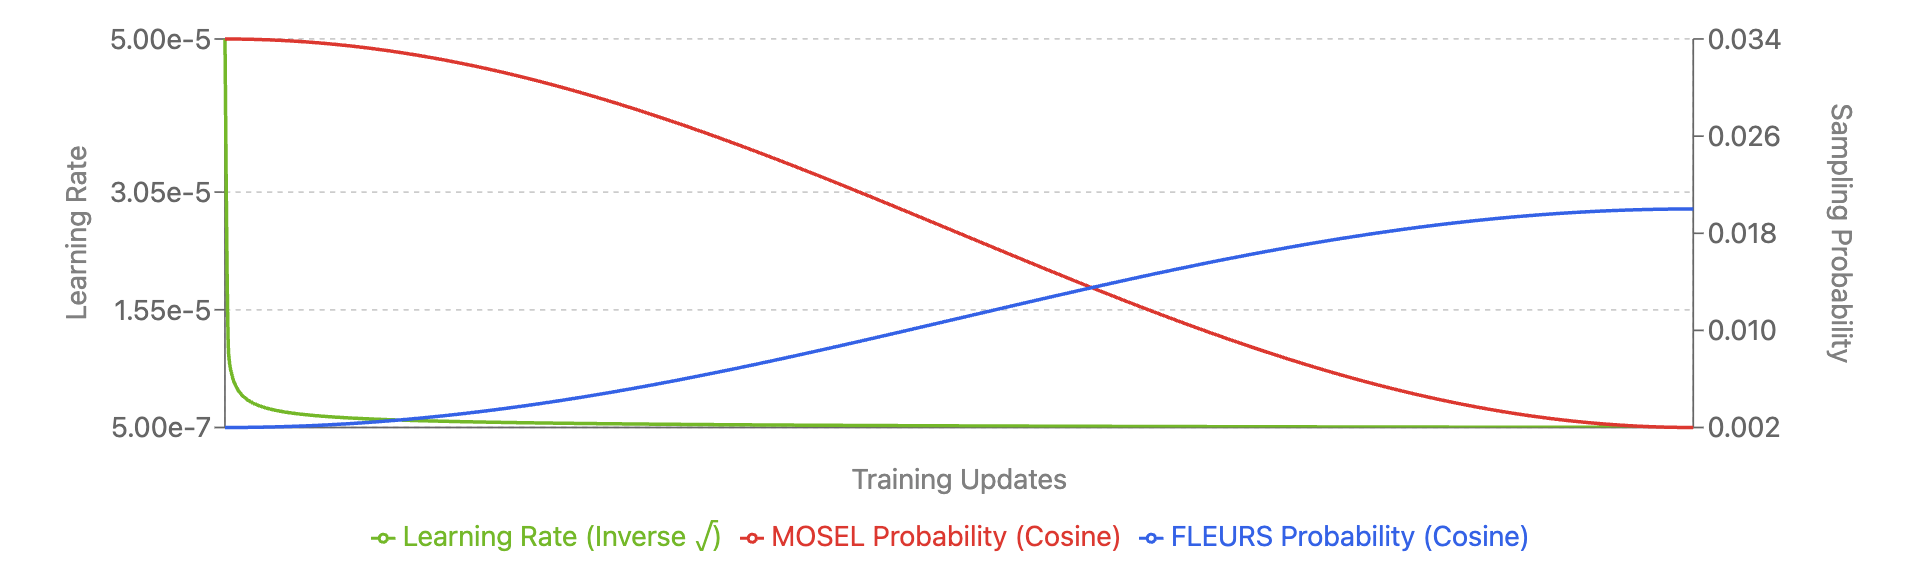
\includegraphics[width=0.9\textwidth]{images/weight_scheduling.png}
    \caption{Example of Data Balancing Schedule. Green line shows the learning rate (inverse square root schedule), while red and blue lines represent MOSEL and FLEURS sampling probabilities (cosine schedules) along the fine-tuning process.}
    \label{fig:weight_scheduling}
\end{figure}

\begin{table}[ht]
\centering
\small
\begin{threeparttable}

% (a) ASR
\begin{subtable}{\textwidth}
\centering
\begin{tabularx}{\textwidth}{l YYYY}
\toprule
\textbf{Model} &
HF Leaderboard (En) & FLEURS (25) & MLS (5) & CoVoST2 (13) \\
\midrule
Pre-trained baseline & 8.36\% & 11.03\% & 7.21\% & 8.31\% \\
\midrule
Fine-tuned (15k HQ) & \textbf{7.15\%} & 8.69\% & \textbf{7.11\%} & 10.33\% \\
Fine-tuned (Balancing schedule) & \textbf{7.15\%} & \textbf{8.40\%} & 7.27\% & \textbf{8.85\%} \\
\bottomrule
\end{tabularx}
\caption{ASR results (WER). Lower is better.}
\end{subtable}

\vspace{10pt} % <-- gap

% (b) AST X->En
\begin{subtable}{\textwidth}
\centering
\begin{tabularx}{\textwidth}{l YY}
\toprule
\textbf{Model} &
FLEURS (24) & CoVoST2 (11) \\
\midrule
Pre-trained baseline & 73.23 & 75.76 \\
\midrule
Fine-tuned (15k HQ) & 79.27 & 76.82 \\
Fine-tuned (Balancing schedule) & \textbf{79.30} & \textbf{77.48} \\
\bottomrule
\end{tabularx}
\caption{AST (X$\to$En) results (COMET). Higher is better.}
\end{subtable}

\vspace{10pt} % <-- gap

% (c) AST En->X
\begin{subtable}{\textwidth}
\centering
\begin{tabularx}{\textwidth}{l YY}
\toprule
\textbf{Model} &
FLEURS (24) & CoVoST2 (5) \\
\midrule
Pre-trained baseline & 83.86 & 80.14 \\
\midrule
Fine-tuned (15k HQ) & 84.38 & \textbf{80.32} \\
Fine-tuned (Balancing schedule) & \textbf{84.56} & 80.29 \\
\bottomrule
\end{tabularx}
\caption{AST (En$\to$X) results (COMET). Higher is better.}
\end{subtable}

\caption{Comparison of pre-trained vs. fine-tuned models across ASR and AST benchmarks.}
\label{tab:asr-ast-finetuning}
\end{threeparttable}
\end{table}

Table~\ref{tab:asr-ast-finetuning} presents the results of these two setups compared to the initial pre-trained checkpoint. Fine-tuning with rebalanced data distribution successfully mitigated narrow-domain and corpus imbalance effects for ASR and X→En tasks. Improvements are particularly visible on the FLEURS dataset, which offers cleaner and more controlled evaluation conditions than CoVoST2. We achieved an ~6 absolute COMET improvement (73.23 → 79.30) for X→En, and a ~25\% relative WER reduction (11.03\% → 8.40\%) for ASR. As expected, En→X performance remained stable across setups, since the original pre-training distribution for this direction was already well-balanced.

Comparing the two fine-tuning strategies, overall performance is similar, with the exception of ASR on CoVoST2, where weight scheduling yielded a 1.5\% absolute WER gain. Since CoVoST2 is the most spontaneous of our benchmarks, we hypothesize that weight scheduling prevents “catastrophic forgetting” of pre-trained knowledge, whereas fine-tuning only on 15k hours of clean data biases the model too strongly toward clearer speech. Moreover, weight scheduling consistently extracted more performance from the available data, leading to additional gains in the X→En direction.

In light of these findings, we release the weight-scheduled fine-tuned model as our primary version and continue to explore data balancing schedules to better understand their benefits and broader applicability.

% \paragraph{Implementation note: Parakeet-TDT-0.6B-v3.}

Fine-tuning stage for \emph{Parakeet-TDT-0.6B-v3} ran for 5,000 steps on 4 A100 GPUs using 7,500 hours of high-quality NeMo ASR Set 3.0 data.



